\clearpage
\thispagestyle{empty}

\movetoevenpage
\small\MyriadPro
\label{colaboradores}

\noindent{}COLABORADORES\\

\noindent{}DANIELA MOUNTIAN é tradutora, designer e criadora da Kalinka, de­dicada
à cultura russa. Fez pela \scalebox{0.8}{USP} graduação em história, mestrado sobre
Fiódor Sologub e doutorado"-sanduíche sobre Daniil Kharms, com estágio de
um ano na Casa de Púchkin, em São Petersburgo. Atualmente é
pós"-doutoranda do Departamento de Teoria Literária e Literatura
Comparada (\scalebox{0.8}{USP}), com apoio da \scalebox{0.8}{FAPESP}. Foi indicada ao prêmio Jabuti pela
tradução de \emph{Os sonhos teus vão acabar contigo}, de Daniil Kharms
(Kalinka, 2013, com Aurora Bernardini e Mois­sei Mountian). Traduziu com
seu pai, Moissei, o conto ``Luz e sombras'', de Sologub, para a
\emph{Nova antologia do conto russo} (Editora 34, 2011), e ``Ivan
Fiódorovitch Chponka e sua titia'', de Nikolai Gógol, para a
\emph{Antologia do humor russo} (Editora 34, 2018); e os livros
\emph{Diário de um escritor (1873): Meia carta de um sujeito}, de Fiódor
Dostoiévski (Hedra, 2016), e \emph{A ressurreição do lariço}
(\emph{Contos de Kolimá 5}), de Varlam Chalámov (Editora 34, 2016).


\medskip

\noindent{}YULIA MIKAELYAN nasceu em Moscou. Fez graduação em Letras na
Universidade Estatal de Moscou Lomonóssov e doutorado sobre Serguei
Dovlátov no Programa em Literatura e Cultura Russa da Universidade de
São Paulo. É professora da Universidade \scalebox{0.8}{MGIMO} de Moscou. Entre 2012 e
2014, ministrou aulas de língua russa na Universidade de São Paulo.
Cotraduziu com Mário Ramos os contos ``Um dia humano'', de A.
Aviértchenko, ``Cartas de Tula'', de B. Pasternak, ``Na rua e em casa'',
de S. Dovlátov, para a \emph{Nova antologia do conto russo (1792--1998)}
(Editora 34, 2011). Traduziu o ensaio ``Quem deve aprender a escrever
com quem, as crianças camponesas conosco ou nós com as crianças
campone­sas?'', de L. Tolstói, para a \emph{Antologia do pensamento
crítico russo} (Editora 34, 2013); o conto ``O coronel diz que eu a
amo'', de Dovlátov, para a \emph{Antologia do humor russo} (Editora 34,
2018); e do mesmo autor o livro \emph{Parque Cultural} (Kalinka, 2016).
Em parceria com Daniela Mountian, verteu ainda \emph{O ofício}, também
de Dovlátov (Kalinka, 2017).

\medskip

\noindent{}MOISSEI MOUNTIAN é tradutor e parte do conselho editorial da Kalinka.

\medskip

\noindent{}PAULO HENRIQUE POMPERMAIER é graduado em Jornalismo pela Faculdade Cásper Líbero e graduando em Letras pela \scalebox{0.8}{USP}. Como repórter atuou na Revista \scalebox{0.8}{\emph{CULT}} e atualmente é editor-assistente da Hedra.

\afterpage{\blankpage}

\newpage
\pagestyle{empty}
\MyriadPro

\noindent{}Catálogo da editora Kalinka\\[5pt]

\noindent{}O Diabo Mesquinho\\
FIÓDOR SOLOGUB
\medskip

\noindent{}Encontros com Liz e outras histórias\\
LEONID DOBÝTCHIN
\medskip

\noindent{}``Os sonhos teus vão acabar contigo'': prosa, poesia, teatro\\
DANIIL KHARMS
\medskip

\noindent{}Luminescência: antologia poética\\
VIATCHESLÁV KUPRIYÁNOV
\medskip

\noindent{}Luminescência: desdobramentos\\
VIATCHESLÁV KUPRIYÁNOV
\medskip

\noindent{}Poesia russa: seleta bilíngue
\medskip

\noindent{}Tarakã, o bigodudo (Ars et Vita e Kalinka)\\
KORNEI TCHUKÓVSKI
\medskip

\noindent{}Parque Cultural\\
SERGUEI DOVLÁTOV
\medskip

\noindent{}Salmo\\
FRIEDRICH GORENSTEIN
\medskip

\noindent{}O ofício\\
SERGUEI DOVLÁTOV
\medskip

\noindent{}O elefante (Coleção Mir)\\
ALEKSANDR KUPRIN
\medskip

\noindent{}A velha (Coleção Mir)\\
DANIIL KHARMS 
\medskip

\noindent{}Bobók \& `Meia carta' de sujeito (Coleção Mir)\\
FIÓDOR DOSTOIÉVSKI
\medskip

\noindent{}Aulas de literatura russa: de Púchkin a Gorenstein \\
AURORA FORNONI BERNARDINI
\medskip

\noindent{}O compromisso\\
SERGUEI DOVLÁTOV

\newpage
\pagestyle{empty}
\MyriadPro
\scriptsize
\begin{center}
KOMPROMISS\\[6pt]

Copyright © 1981, Sergei Dovlatov\\[6pt]

All rights reserved\\[20pt]

Copyright © Kalinka, 2019\\[6pt]

Tradução © Daniela Mountian, Yulia Mikaelyan, 2019\\[6pt]

Posfácio © Daniela Mountian, Yulia Mikaelyan, 2019\\[6pt]

primeira edição, 2019\\[40pt]


Essa publicação está de acordo com a reforma ortográfica.\\[6pt]
A versão se baseou no livro \emph{Serguei Dovlátov, sobránie sotchiniéni} (São Petersburgo, \emph{Ázbuka}, 2018).\\[6pt]	
A imagem que precede o posfácio é baseada em autocharge do autor.\\[20pt]
\end{center}


\bigskip

\begin{vplace}[1]
\begin{table}[ht!]
\MyriadPro
\scriptsize
\begin{tabular}{rl}
TÍTULO            & O compromisso 									   \\[2pt]
AUTOR             & Serguei Dovlátov                          		   \\[2pt]
TRADUÇÃO do RUSSO & Daniela Mountian                                   \\[2pt]
TRADUÇÃO do RUSSO & Yulia Mikaelyan 	 			                   \\[2pt]
COTEJO            & Moissei Mountian 							       \\[2pt]
REVISÃO           & Paulo Henrique Pompermaier                         \\[2pt]
CAPA              & Daniela Mountian                                   \\[2pt]
PROJETO GRÁFICO   & Kalinka                                            \\[2pt]
PRODUÇÃO EXECUTIVA & Hedra                                             \\[2pt]
EDIÇÃO            & kalinka 		                                   \\[2pt] 
FORMATO           & 14 x 21 cm                                         \\[2pt]
NÚMERO de PÁGINAS & XXX                                                \\[2pt]
ISBN              & 978-85-61096-XX-X                                 
\end{tabular}
\end{table}
\end{vplace}

\newpage
\MyriadPro
\begin{center}
\small
Compromisso

Компромисс
\end{center}

\scriptsize


\begin{figure}[!ht]
%\begin{minipage}{2\textwidth}
\centering

  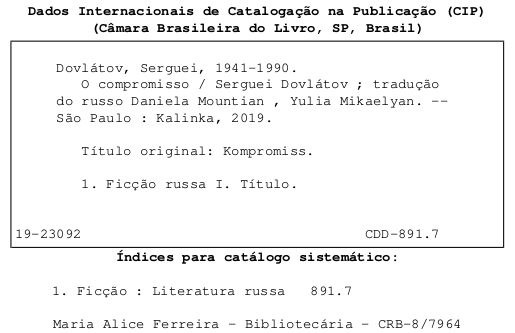
\includegraphics[width=80mm]{./imgs/ficha.jpg}
%\caption{I}
%\end{minipage}
 \end{figure}


%\begin{vplace}[1]
%\begin{center}
%Dados Internacionais de Catalogação na Publicação (CIP)\\
%(Câmara Brasileira do Livro, SP, Brasil)\\
%\_\_\_\_\_\_\_\_\_\_\_\_\_\_\_\_\_\_\_\_\_\_\_\_\_\_\_\_\_\_\_\_\_\_\_\_\_\_\_\_\_\_\_\_\_\_\_\_\_\_\_\_\_\_\_\_\_\_\_\\
%\end{center}
%\hspace{30pt}Bernardini, Aurora Fornoni, XXXX--


%\hspace{35pt}Aulas de literatura russa : de Púchkin a Gorenstein / Aurora Fornoni

%\hspace{12pt}Bernardini ; organização Valteir Vaz ; prefácio Arlete Cavaliere. - - São Paulo :

%\hspace{12pt}Kalinka, 2018.\\[6pt]

%\hspace{35pt}ISBN XXX-XX-XXXXX-XX-X\\[6pt]

%\hspace{35pt}1. Literatura russa II. Crítica literária III. Título.

%\begin{center}
%\hspace{10pt}XX-XXXXX \hspace{180pt}CDD-XXX.X
%\_\_\_\_\_\_\_\_\_\_\_\_\_\_\_\_\_\_\_\_\_\_\_\_\_\_\_\_\_\_\_\_\_\_\_\_\_\_\_\_\_\_\_\_\_\_\_\_\_\_\_\_\_\_\_\_\_\_\_\\
%Índices para catálogo sistemático:\\[3pt]
%1. Crítica literária : Literatura russa XXX.X\\
%\end{center}
%\end{vplace}
\vfill
\begin{center}
EDIÇÃO: EDITORA KALINKA\\[7pt]
Rua Imaculada Conceição, 41 cj. 03\\[7pt]
01226-020 São Paulo-SP Tel.11 2579-6290\\[7pt]
www.kalinka.com.br\\[30pt]

PRODUÇÃO EXECUTIVA: EDITORA HEDRA\\[7pt]
Rua Fradique Coutinho, 1139 Vila Madalena\\[7pt]
05416-011 São Paulo-SP Tel.11 3097-8304\\[7pt]
www.hedra.com.br
\end{center}

%TÍTULO Aulas de literatura russa: de Púchkin a Gorenstein\\
%AUTOR Aurora Fornoni Bernardini\\
%REVISÃO Daniela Mountian e Paulo Henrique Pompermaier\\
%EDIÇÃO Hedra\\
%CAPA Daniela Mountian\\
%PROJETO GRÁFICO Hedra\\
%FORMATO 14 x 21 cm\\
%NÚMERO de PÁGINAS 398\\
%ISBN XXX-XX-XXXXX-XX-X\\